% Filename  : samplepaper.tex
% Purpose   : A sample exam paper to demonstrate how to use the 'ditpaper'
%             TeX class.
% Author    : Emmet Caulfield
% Revision  : $Id: samplepaper.tex 2 2006-02-19 20:34:45Z emmet $
% Repository: $HeadURL: http://svn.netrogen.lan/tex-ditpaper/trunk/samplepaper.tex $
%

% 'nosolution' (default) and 'solution' toggle the inclusion of solutions
% in the output. The tag --SOLUTION-OPTION--, below, is replaced by 'sed' 
% in the Makefile to cause both the paper and the solutions to be produced.
\documentclass[--SOLUTION-OPTION--]{ditpaper}

\usepackage{graphicx}

% These must be set or bizarre defaults will be used:
\facility{Kevin Street, Dublin 8}
\course{BSc (Hons) in Computer Science}
\examcode{S228/406}
\stage{Stage 4}
\session{Semester 2 Examinations 2008}
\title{Artificial Intelligence 2}
\examiners{Dr. John Kelleher\\
Prof. B. O'Shea\\
Dr. I. Arena}
\examdate{}
\examtime{Duration: 2 Hours}
\instructions{Answer Question 1 (40 marks) \textbf{and}\par{} any 2 Other Questions (30 marks each).}

\begin{document}

% questions from across the course
\question
\begin{enumerate}
	\item Distinguish between \textbf{supervised} and \textbf{unsupervised} learning.
		\marks{5}
		\begin{answer}
			The distinction is that with \textbf{supervised learning} we know the actual label or category for each piece of data on which we train, whereas with \textbf{unsupervised learning} we do not know the classification of the data in the training sample. Unsupervised learning can thus often be viewed as a \textbf{clustering} task, while supervised learning can usually be seen as a \textbf{classification} task, or equivalently as a function-fitting task where one extrapolates the shape of a function based on some data points.
		\end{answer}
	\item In the context of machine learning, explain what is meant by \textbf{overfitting} the training data.	
		\marks{5}
		\begin{answer}
			Overfitting occurs when classifiers make decisions based on accidental properties of the training set that will lead to errors on the test set (or new data). As a result, whenever there is a large set of possible hypotheses, one has to be careful not to use the resulting freedom to find meaningless "regularity" in the data.
		\end{answer}
	\item Explain what is meant by the term \textbf{abductive reasoning}.
		\marks{5}
		\begin{answer}
		Abductive reasoning allows the antecedent (head) of a rule to concluded with the conclusion is true provided that doing so is consistent. Abductive reasoning is primarily diagnostic; given the effect find the likely cause.
		\end{answer}
	\item What does it mean if two classes $C_1$ and $C_2$ are described as \textbf{linearly separable}.	
		\marks{5}
		\begin{answer}
		This means that for each class $C_i$ there exists a hyperplane $H_i$ such that on its positive side lie all $x \in C_i$ and on its negative side lie all $x \in C_j , j \ne i$
		\end{answer}
	\item Let us say we have three classification algorithms. How can we order these three from best to worst?
		\marks{20}
		\begin{answer}
		This is a discursive question so giving a precise answer is not appropriate. However, key points that the student should touch on include:
		\begin{itemize}
			\item Predictive accuracy
			\item Speed and scalability 
				\begin{itemize}
					\item Time to construct the model
					\item Time to use the model
				\end{itemize}
			\item Robustness (handling noise and missing values)
			\item Scalability
			\item Interpretability (understanding and insight provided by the model)
		\end{itemize}
		it should be noted also, that these evaluation criteria are application dependent.
		\end{answer}
\end{enumerate}



%Q2 30 marks
% reasoning under uncertainty
% aima chapters 13, 14, 15
\question
\begin{enumerate}
	%aima
	\item In your local power station, there is an alarm that senses when a temperature gauge exceeds a given threshold. The gauge measures the temperature of the core. Consider the Boolean variables $A$ (alarm sounds), $F_A$ (alarm is faulty), and $F_G$ (gauge is faulty) and multivalued nodes $G$ (gauge reading) and $T$ (actual core temperature).
	\begin{enumerate}
		\item Draw a Bayesian network for this domain, given that the gauge is more likely to fail when the core temperature gets too high.
		\marks{5}
		\begin{answer}
		The key aspects are: the failure nodes are parents of the sensor nodes, and the temperature node is a par ent of both the gauge and the gauge failure node. It is exactly this kind of correlation that makes it dif�cult for humans to understand what is happening in complex systems with unreliable sensors.
		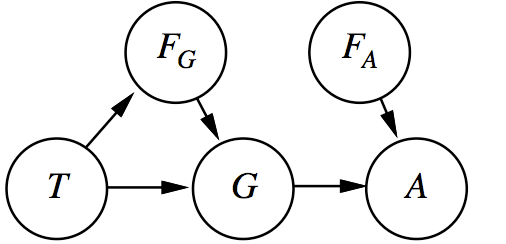
\includegraphics[width=\textwidth]{./images/nuclearpowerstationbayesiannet.png}
		\end{answer}
		\item Suppose there are just two possible actual and measured temperatures: normal and high. The probability that the gauge gives the correct temperature is $x$ when it is working, but $y$ when it is faulty. Give the conditional probability table associated with node $G$.
		\marks{5}
		\begin{answer}
		Note the semantics of $F_G$ , which is true when the gauge is faulty, i.e., not working.
		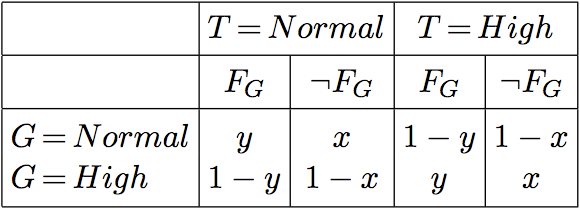
\includegraphics[width=\textwidth]{./images/cpt_node_g_q142.png}
		\end{answer}
		%\item I have left out the rest of this question fill it in when I get a chance - the CPTs for part 2 and 3 are in the images folder.
	\end{enumerate}
	\item After your yearly checkup, the doctor has bad news and good news. The bad news is that you tested positive for a serious disease and that the test is $99\%$ accurate (i.e., the probability of testing positive when you do have the disease is 0.99, as is the probability of testing negative when you don't have the disease). The good news is that this is a rare disease, striking only 1 in 10,000 people of your age. 
	\begin{enumerate}
		\item Why is it good news that the disease is rare? 
			\marks{10}
			\begin{answer}
 				What the patient is concerned about is $P(disease|test)$. Now $P(a|b) = \frac{P(b|a)P(a)} {P(a)}  \rightarrow P(disease|test) = \frac{P(test|disease)P(disease)}{P(test)}\rightarrow$ roughly speaking, the reason it is a good thing that the disease is rare is that $P(disease|test)$ is proportional to $P(disease)$, so a lower prior for disease will mean a lower value for $P(disease |test)$. Roughly speaking, if 10,000 people take the test, we expect 1 to actually have the disease, and most likely test positive, while the rest do not have the disease, but 1 percent of them (about 100 people) will test positive anyway, so $P(disease |test)$ will be about 1 in 100.  The moral is that when the disease is much  rarer than the test a ccuracy, a positive test result does not mean the disease is likely. A false positive reading remains much more likely. 
		\end{answer}
		\item What are the chances that you actually have the disease?
			\marks{10}
			\begin{answer}
				We are given the following information: 
				$P (test | disease) = 0.99$ \\
				$P ( \lnot test | \lnot disease) = 0.99$\\ 
				$P (disease) = 0.0001$\\
				and the observation $test$.\\
				$P(a|b) = \frac{P(b|a)P(a)} {P(a)} $ \\
				$P(disease|test) = \frac{P(test|disease)P(disease)}{P(test)}\rightarrow$\\
				$P(disease|test) = \frac{P(test|disease)P(disease)}{P(test|disease)P(disease)+P(test|\not disease)P(\lnot disease)}\rightarrow$\\
				$\frac{0.99 \times 0.0001}{(0.99 \times 0.0001)+(0.1 \times 0.9999)}$\\
				$P(disease|test)=.009804$
			\end{answer}
	\end{enumerate}
\end{enumerate}
 
\newpage

%Q3
%Inductive Learning (Decision Trees)
%aima chapters 18
\question
\begin{enumerate}
	\item In the context of Decision Tree Learning define what is meant by the following terms:
		\begin{enumerate}
			%Callan
			\item entropy
				\marks{5}
				\begin{answer}
				For $c$ classification categories the entropy $E$ is defined as: $E=\sum_{i=1}^{c} -p_i\ log_2\ p_i$ where $p_i$ is the probability of category $i$ occurring.
				\end{answer}
			%Callan
			\item information gain
				\marks{5}
				\begin{answer}
				The information gain for an attribute is the expected reduction in entropy if the examples were to be partitioned according to that attribute and is defined as: $Gain(T,A)=E(T) - \sum_{j=1}^{v} \frac{|T_{j}|}{|T|}E(T_{j})$ where $T$ is a set of training examples and $T_j$ is a subset of examples having value $j$ for attribute $A$ 
				\end{answer}
		\end{enumerate}
	%aima Q18.4
	\item Using the ID3 algorithm we never test the same attribute twice along one path in a decision tree. Why not?
				\marks{5}
				\begin{answer}
				In standard decision trees, attribute tests divide examples according to the attribute value. Therefore any example reaching the second test already has a known value for the attribute and the second test is redundant. In some decision tree systems, however, all tests are Boolean even if the attributes are multivalued or continuous. In this case, additional tests of the attribute can be used to check different values or subdivide the range further (e.g., �rst check if $X > 0$, and then if it is, check if $x > 10$). 
				\end{answer}
			%Q18.5
	\item Suppose we generate a training set from a decision tree and then apply decision-tree learning to the training-set. Is it the case that the learning algorithm will eventually return the correct tree as the training set size goes to infinity? Why or why not?
				\marks{5}
				\begin{answer}
				The algorithm may not return the''correct'' tree, but it will return a tree that is logically equivalent, assuming that the method for generating examples eventually generates all possible combinations of input attributes. This is true because any two decision tree defined on the same set of attributes that agree on all possible examples are, by de�nition, logically equivalent. The actual form of the tree may differ because there are many different ways to represent the same function. (For example, with two attributes A and B we can have one tree with $A$ at the root and another with $B$ at the root.) The root attribute of the original tree may not in fact be the one that will be chosen by the information gain heuristic when applied to the training examples. 
				\end{answer}
	\item Discuss the advantages and disadvantages of \textbf{$k$-Nearest Neighbour} classification.
				\marks{10}
				\begin{answer}
				Strengths
				\begin{enumerate}	
					\item No training involved � lazy learning
					\item New data can be added on the fly
					\item Some explanation capabilities
					\item Robust to noisy data by averaging k-nearest neighbors
				\end{enumerate}
				Weaknesses
				\begin{enumerate}
					\item Not the most powerful classification (generally its accuracy will be lower than an ANN or SVM model)
					\item Slow classification 
					\item Curse of dimensionality (as you increase the number of features you need more and more examples to cover the problem space - kNN are particularly susceptible to this issue as they do not do any feature selection).
				\end{enumerate}
			\end{answer}	
\end{enumerate}
 
%Q4
%Neural Nets
\question Figure \ref{fig:nn} shows a backprogation network that is currently processing the training vector $[1.0, 0.9, 0.9]$ which has an  associated target vector $[0.1, 0.9, 1.0]$. Given that the output from unit B is $0.6$ and from C is $0.8$, and assuming that the activation function used at all nodes in the network is the logistic function (i.e., $f(x) = \frac{1}{1 + \exp^{-x}}$): 
\begin{enumerate}
	\item Calculate the actual output vector (to 3 decimal places).
		\marks{5}
		\begin{answer}
		Output of unit $i = f(\sum_{j=1}^{n}W_{j,i}\times activation_j)$\\
		First output unit input = -0.3 x 0.6 + 0.9 x 0.8 = 0.54 $\rightarrow$ f(0.54) = 0.632\\
		Second output unit input = -0.6 x 0.6 + -0.1 x 0.8 = -0.44 $\rightarrow$ f(-0.44) = 0.392\\
		Third output unit input = 0.4 x 0.6 + 1.2 x 0.8 = 1.2 $\rightarrow$ f(1.2)= 0.769\\
		\end{answer}
	\item Calculate the error for each output unit.
		\marks{5}
		\begin{answer}
		Error =  target - output\\
		First output unit = (0.1 - 0.632)  = - 0.532\\
		Second output unit = (0.9 - 0.392) = 0.508\\
		Third output unit = (0.1 - 0.769) = - 0.696\\
		\end{answer}
	\item Calculate the error for each hidden unit B and C.
		\marks{10}
		\begin{answer}
		Each hidden node $j$ is responsible for some fraction of the error $Err_i$ of each of the output units $i$ to which it connects. Thus the $Err_i$ values are divided according to the strengths of the connection between the hidden node and the output nodes and are propagated back to the hidden nodes. Where a hidden node feeds-forward into more than 1 output node the errors propagated back to it are summed: $Err_j = \sum_{i=1}^{n}W_{ji} \times Err_i$:
		$Err_{B} = (-0.3 \times -0.532) + (-0.6 \times 0.508) + (0.4 \times -0.696) = 0.1596 + -0.3048 + -0.2784 = -0.4236$\\
		$Err_{C} = (0.9 \times -0.532) + (-0.1 \times 0.508) + (1.2 \times -0.696) =  -0.4788 + -0.0508 + -0.8352  = -1.3648$\\
		\end{answer}
	\item Calculate the new weight for the connection from unit B to the output unit D after the training example has been processed. Use a learning rate of $\alpha = 0.25$ and momentum of zero.
		\marks{10}
		\begin{answer}
			The weight  update rules is:\\
			$W_{j,i} = W_{j,i} + (\alpha \times activation_j \times Err_i \times \frac{\delta f(e_i)}{\delta e_i})$\\
			where $e_i =\sum_{j=0}^{n}W_{j,i} \times activation_j)$ and $f()$ is the network activation function. When $f(e_i)$ is a sigmoidal function (as in this question) $\frac{\delta f(e_i)}{\delta e_i}= f(e_i) \times (1-f(e_i))$.\\
		From part 1 $e_D = 0.54$ and $f(e_D) = 0.3682$\\
		$W_{B,D} = W_{B,D} + (\alpha \times activation_B \times Err_D \times f(e_D) \times (1 + f(e_D) \rightarrow$\\
		$W_{B,D} = -0.3         + (0.25     \times 0.6                \times  -0.532 \times 0.632 \times (1+ 0.632)) \rightarrow$\\
		$W_{B,D} = -0.3         + (0.25     \times 0.6                \times  -0.532 \times 0.632 \times (1.632)) \rightarrow$\\
		$W_{B,D} = -0.3         + (0.25     \times 0.6                \times  -0.532 \times 1.031424) \rightarrow$\\
		$W_{B,D} = -0.3         + (0.25     \times 0.6                \times -0.548717568) \rightarrow$\\
		$W_{B,D} = -0.3         + (0.25     \times -0.3292305408) \rightarrow$\\
		$W_{B,D} = -0.3         + (-0.0823076352) \rightarrow$\\
		$W_{B,D} = -0.3823076352 \rightarrow$\\
		$W_{B,D} = -0.3823 $ rounded\\
	\end{answer}
\end{enumerate}

\begin{figure}[htbp]
\begin{center}
\includegraphics[width=3.5in]{./images/nn_callan_q10_2.png}
\caption{Example Neural Net}
\label{fig:nn}
\end{center}
\end{figure}


\end{document}
